\documentclass[danish,a4paper]{report}
\usepackage[T1]{fontenc}
\usepackage[utf8]{inputenc}
\usepackage{lmodern}
\usepackage{hyperref}
\usepackage{graphicx}
\usepackage[english]{babel}
\usepackage{verbatim}
\usepackage{color}
\usepackage[table]{xcolor}
\usepackage{graphicx}
\usepackage{amsmath}

\usepackage{tikz}
\usetikzlibrary{automata,positioning}

\usepackage{parskip}
\usepackage{url}
\usepackage{background}
\usepackage{lastpage}
\usepackage{titlesec}
\usepackage{blindtext}
\usepackage{color}
\usepackage{nopageno}
\usepackage{todonotes}
\usepackage{listings}

\definecolor{dkgreen}{rgb}{0,0.6,0}
\definecolor{gray}{rgb}{0.5,0.5,0.5}
\definecolor{mauve}{rgb}{0.58,0,0.82}
\definecolor{gray75}{gray}{0.75}
\definecolor{light-gray}{gray}{0.5}

\lstset{
  frame=,
  language=C,
  aboveskip=3mm,
  belowskip=3mm,
  showstringspaces=false,
  columns=flexible,
  basicstyle={\small\ttfamily},
  numbers=none,
  numberstyle=\tiny\color{gray},
  keywordstyle=\color{blue},
  commentstyle=\color{dkgreen},
  stringstyle=\color{mauve},
  breaklines=true,
  breakatwhitespace=true
  tabsize=4
}

\addtolength{\topmargin}{-1.5cm}
\addtolength{\textheight}{1.5cm}
\addtolength{\oddsidemargin}{-1cm}
\addtolength{\evensidemargin}{-1cm}
\addtolength{\textwidth}{2cm}

 
\definecolor{schultz}{RGB}{146,34,126}
\definecolor{gray75}{gray}{0.75}
\definecolor{light-gray}{gray}{0.5}
\newcommand{\hsp}{\hspace{20pt}}
\titleformat{\chapter}[hang]{\Huge\bfseries}{\thechapter\hsp}{0pt}{\Huge\bfseries}[{\titlerule[1.5pt]}]
% \titlespacing*{\chapter}{0cm}{-10pt}{2em}
\titlespacing*{\chapter}{0cm}{-20pt}{2em}
\setcounter{secnumdepth}{3}
\setcounter{tocdepth}{1}

\titlespacing*{\section} {0pt}{5pt}{2pt}
\titlespacing*{\subsubsection}{0pt}{0pt}{0pt}

\backgroundsetup{
  scale=1,
  color=black,
  opacity=1,
  angle=0,
  position=current page.south,
  vshift=60pt,
  contents={%
  \small%
  \begin{minipage}{.48\textwidth}
  \vspace{-2cm}
  \parbox[b]{.4\textwidth}{%
    Side \thepage\ af \pageref{LastPage}}\hfill
  \parbox[b]{.6\textwidth}{%
  \raggedleft \titlename}
  \rule{\textwidth}{1.5pt}\\
  \parbox[b]{.7\textwidth}{%
      \name }\hfill
  \parbox[b]{.3\textwidth}{%
  \raggedleft \email } 
  \end{minipage}\hspace{.02\textwidth}%
  \begin{minipage}{.5\textwidth}
  \vspace{-2cm}
  \includegraphics[width=\linewidth,height=70pt,keepaspectratio]{footer_logo}
  \end{minipage}%
  }
}

\newcommand{\namesigdate}[2][10cm]{%
  \begin{tabular}{@{}p{#1}@{}}
    #2 \\[2\normalbaselineskip] \hrule \\[0pt]
    {\small \textit{Signature}} \\[2\normalbaselineskip] \hrule \\[0pt]
    {\small \textit{Date}}
  \end{tabular}
}

\newcommand{\titlename}{Programmer som Data}
\newcommand{\name}{Jacob Benjamin Cholewa}
\newcommand{\email}{jbec@itu.dk}


\makeatletter
\NoBgThispage
 \title{\Huge \textbf{\titlename}\\\huge Eksamens opgave Januar 2015}
 % Author
\author{\textsc{\name} \\ \textsc{\email}}
\begin{document}
\maketitle

\vspace*{\fill}
\begin{center}
\begin{large}
Jeg erklærer hermed at jeg selv har lavet hele denne eksamensbevarelse uden hjælp fra andre
\end{large}

\vspace*{2cm}
\namesigdate{}
\end{center}

\vspace*{\fill}


\newpage

\chapter*{Opgave 1}
\section*{Spørgsmål 1.1}
Det regulære udtryk $e(fd*)*x$ beskriver et bar system. Du kan gå ind i baren, $e(nter)$, og her kan du så hente øl, $f(etch)$, (Du behøver ikke). Når du har en øl kan du hente en mere eller du kan drikke af den du allerede har 0 til flere gange $d(rink)$. Tilsidst kan du gå ud af baren, $e(xit)$, lige gyldigt om du har eller ikke har hentet og drukket øl.

Dette regulære udtryk beskriver altså for eksempel disse strenge:
\begin{center}$ ex$,
$efx$,
$effx$,
$efdx$,
$efffdx$,
$efddfddfx$
\end{center}
hvor disse strenge ville være ugyldige:
\begin{center}
$fx$,
$fdx$,
$efd$,
$edx$
\end{center}
\section*{Spørgsmål 1.2}
\label{sec:sp2}

Jeg har i dette spørgsmål konstrueret en NFA ved hjælp af en systematisk konstruktion som vist i undervisningen og i \textit{Converting Reguler Expressions to Discrete Finite Automata: A tutorial} af David Christiansen\\

\begin{center}
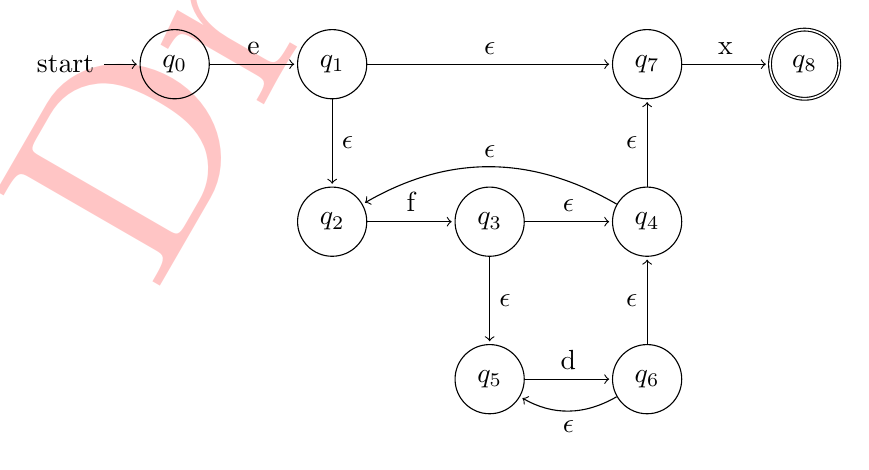
\begin{tikzpicture}[shorten >=1pt,node distance=2cm,on grid,auto] 
   \node[state,initial]   (q_0)                         {$q_0$}; 
   \node[state]           (q_1) [right=of q_0]          {$q_1$};
   \node[state]           (q_2) [below=of q_1]          {$q_2$}; 
   \node[state]           (q_3) [right=of q_2]          {$q_3$}; 
   \node[state]           (q_4) [right=of q_3]          {$q_4$}; 
   \node[state]           (q_5) [below=of q_3]          {$q_5$}; 
   \node[state]           (q_6) [right=of q_5]          {$q_6$}; 
   \node[state]           (q_7) [above=of q_4]          {$q_7$}; 
   \node[state,accepting] (q_8) [right=of q_7]          {$q_8$}; 


    \path[->] 

    (q_0) edge              node {e}           (q_1)
    (q_1) edge              node {$\epsilon$}  (q_7)
          edge              node {$\epsilon$}  (q_2)
    (q_2) edge              node {f}           (q_3)
    (q_3) edge              node {$\epsilon$}  (q_4)
          edge              node {$\epsilon$}  (q_5)
    (q_4) edge              node {$\epsilon$}  (q_7)
          edge [bend right] node [swap ]{$\epsilon$}  (q_2)
    (q_5) edge              node {d}           (q_6)
    (q_6) edge [bend left]  node {$\epsilon$}  (q_5)
          edge              node {$\epsilon$}  (q_4)
    (q_7) edge              node {x}           (q_8);
\end{tikzpicture}
\end{center}
\newpage
\section*{Spørgsmål 1.3}

Jeg har i denne opgave brugt en systematisk tilgang til at oversætte min NFA vist i spørgsmål 2. Det første jeg gør er at prøve at fjerne alle $\epsilon$ overgange. Det kan jeg opnå ved at lave en DFA hvor hver stadie svare til et sæt stadier fra den gamle NFA. Et nyt stadie i DFA'en svare til et stadie og alle de stadier som kan nås med $\epsilon$ overgange fra det første stadie. I tabellen neden for viser jeg de nye DFA stadier, hvilke overgange de har til andre stadier og hvilke gamle NFA stadier de svare til.
\begin{table}[h]
\centering
\begin{tabular}{|l|l|l|l|l|l|}
\hline
State      & e   & f   & d   & x      & NFA States                            \\ \hline
$S_0$      & $S_1$  & -      & -      & -     & $\{q_0\}$                     \\
$S_1$      & -      & $S_3$  & -      & $S_2$ & $\{q_1, q_2, q_7\}$           \\
$S_2$      & -      & -      & -      & -     & $\{q_8\}$                     \\
$S_3$      & -      & $S_3$  & $S_4$  & $S_2$ & $\{q_2, q_3, q_4, q_5, q_7\}$ \\
$S_4$      & -      & $S_3$  & $S_4$  & $S_2$ & $\{q_2, q_4, q_5, q_6, q_7\}$ \\ \hline
\end{tabular}
\end{table}

Derefter har jeg tegnet en DFA svarende til tabellen

\begin{center}
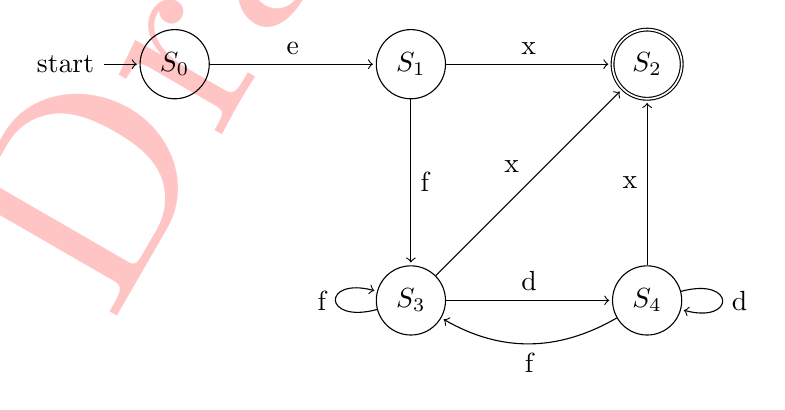
\begin{tikzpicture}[shorten >=1pt,node distance=3cm,on grid,auto] 
   \node[state,initial]   (s_0)                         {$S_0$}; 
   \node[state]           (s_1) [right=of s_0]          {$S_1$};
   \node[state,accepting] (s_2) [right=of s_1]          {$S_2$}; 
   \node[state]           (s_3) [below=of s_1]          {$S_3$}; 
   \node[state]           (s_4) [right=of s_3]          {$S_4$}; 


    \path[->] 

    (s_0) edge                node          {e} (s_1)
    (s_1) edge                node          {x} (s_2)
          edge                node          {f} (s_3)
    (s_3) edge  [loop left]   node          {f} (s_3)
          edge                node          {d} (s_4)
          edge                node          {x} (s_2)
    (s_4) edge  [loop right]  node          {d} (s_4)
          edge  [bend left]   node          {f} (s_3)
          edge                node          {x} (s_2)
          ;

\end{tikzpicture}
\end{center}
\section*{Spørgsmål 1.4}

Jeg er lidt i tvivl om hvordan dette sprog skal tolkes. Jeg går derfor i opgaven ud fra at man skal \textit{fetch beer} før man kan \textit{drink beer} og \textit{spill beer}. Jeg går ud fra at man kun må \textit{fetch beer} \textbf{én} gang da det ikke vises i nogle af eksemplerne at der hentes mere end en øl. Ved denne forståelse kan man danne dette regulære udtryk for sproget:

\begin{align*}
f[sd]*
\end{align*}

\chapter*{Opgave 2}
\section*{Spørgsmål 2.1}

I denne opgave har jeg implementeret \texttt{Pair, Fst} og \texttt{Snd} til den abstrakte syntaks for HigherFun sproget. Dette har jeg gjort ved at ændre i \texttt{absyn.fs} og udvide \texttt{expr} typen. Der vises her kun et udsnit af \texttt{expr} typen.

\begin{lstlisting}[language=ML]
type expr = 
  | Pair of expr * expr
  | Fst of expr 
  | Snd of expr 
  ...
\end{lstlisting}

\section*{Spørgsmål 2.2}

I denne opgave bygger jeg videre på opgave 2.1 og udvider nu \texttt{HigherFun.fs} til at kunne bruge den udvidede abstrakte syntaks. Når et udtryk evalueres i vores lille funktionelle sprog returneres en værdi med typen \texttt{value}. Jeg har nu udvidet \texttt{value} typen med \texttt{ValuePair}, altså et par af værdier, så vi kan evaluere det nye \texttt{Pair} udtryk

\begin{lstlisting}[language=ML]
type value = 
  | Int of int
  | ValuePair of value * value
  | Closure of string * string * expr * value env
\end{lstlisting}

Derefter har jeg ændret i evaluerings logikken så der nu kan evalueres udtryk med \texttt{Pair, Fst} og \texttt{Snd}. Der vises her kun et lille del af evaluerings logikken. Som det kan ses evaluerer vi \texttt{Pair} ved både at evaluere \texttt{e1} og \texttt{e2} til et \texttt{ValuePair}. Jeg bruger \textit{Pattern Matching} til at evaluere \texttt{Fst} og \texttt{Snd} udtryk og sørger samtidig for at det kun er den del af parret man bruger der bliver evalueret. Hvis \texttt{Fst} og \texttt{Snd} bliver kaldt med andet end et \texttt{Pair} som indre udtryk vil de ikke blive \textit{matched} og programmet vil fejle med beskeden \textit{Invalid syntax}


\begin{lstlisting}[language=ML]
let rec eval (e : expr) (env : value env) : value =
    match e with
    ...
    | Pair(e1,e2)     -> ValuePair((eval e1 env),(eval e2 env)) 
    | Fst(Pair(e1,e2))  -> eval e1 env
    | Snd(Pair(e1,e2))  -> eval e2 env
    ...
    | _                 -> failwith "Invalid syntax"
\end{lstlisting}

Jeg tolker i denne opgave ``Bemærk at \texttt{Fst} og \texttt{Snd} skal fejle, hvis værdien de anvendes på ikke er et parudtryk.'' som at jeg kun skal kunne tolke udtryk som

\begin{lstlisting}[language=ML]
let ex = Snd(Pair (CstI 1,Pair (CstI 2,CstI 3)))
\end{lstlisting}

og ikke

\begin{lstlisting}[language=ML]
let ex = Fst(Snd(Pair (CstI 1,Pair (CstI 2,CstI 3))))
\end{lstlisting}

Jeg forklare i Spørgsmål 2.3 hvad det betyder for funktionaliteten og hvordan man kunne have implementeret \texttt{eval} så den kunne evaluere udtryk som det sidste 

\section*{Spørgsmål 2.3}

Jeg har brugt et lille hjælpe program \texttt{run} som kan findes i appendiks. Filen \texttt{ex23} som indeholder mine eksempler kan også findes i appendiks A.

\begin{lstlisting}[language=bash]
$ ./run < ex23
  ...
> val ex1 : expr = Pair (CstI 1,Pair (CstI 2,CstI 3))
> val ex2 : expr = Fst (Pair (CstI 1,Pair (CstI 2,CstI 3)))
> val ex3 : expr = Snd (Pair (CstI 1,Pair (CstI 2,CstI 3)))
> val ex4 : expr =
  Let
    ("x",CstI 3,
     Pair
       (Letfun ("f","x",Prim ("*",Var "x",CstI 2),Call (Var "f",Var "x")),
        Letfun ("f","x",Prim ("+",Var "x",CstI 2),Call (Var "f",Var "x"))))

> val res1 : value = ValuePair (Int 1,ValuePair (Int 2,Int 3))
> val res2 : value = Int 1
> val res3 : value = ValuePair (Int 2,Int 3)
> val res4 : value = ValuePair (Int 6,Int 5)
\end{lstlisting}

Min implementation fungere, men et valg jeg træf var at gøre så \texttt{Fst} og \texttt{Snd} kun evaluere den del af parret som der er brug for. Det gør så også at min implementation ikke kan evaluere udtryk som disse:

\begin{lstlisting}[language=ML]
let ex5 = Snd(Snd(ex1));;
let ex6 = Fst(ex4);;
\end{lstlisting}

Ved at implementere metoden på denne måde kunne man have evalueret udtryk som \texttt{ex5} og \texttt{ex6}, men så bliver man nødt til at evaluere hele parret hvilke ikke gøres i den nuværende implementation.

\begin{lstlisting}[language=ML]
let rec eval (e : expr) (env : value env) : value =
    match e with
    ...
    | Pair(e1,e2)     -> ValuePair((eval e1 env),(eval e2 env)) 
    | Fst(e)  ->  match eval e env with
                  | ValuePair(v1,v2)  -> v1
                  | _                 -> failwith "not a pair"
    | Snd(e)  ->  match eval e env with
                  | ValuePair(v1,v2)  -> v2
                  | _                 -> failwith "not a pair" 
    ...
    | _                 -> failwith "Invalid syntax"
\end{lstlisting}

\section*{Spørgsmål 2.4}

I denne opgave har jeg udvidet parser og lexer specifikationen til at indeholde de tre nye udtryk \texttt{Pair, Fst} og \texttt{Snd} med syntaksen

\begin{lstlisting}[language=ML]
(1,true)
fst(1,true)
snd(1,true)
\end{lstlisting}

Det første jeg har gjort er at tilføje de nye keywords og token. Parenteser er allerede lagt ind som tokens. 

\begin{lstlisting}[language=ML]
let keyword s =
    match s with
    ...
    | "fst"   -> FST
    | "snd"   -> SND
    | _       -> NAME s 

...

rule Token = parse
  ...
  | ','             { COMMA }
  ...
\end{lstlisting}

Derefter udvider jeg parser specifikationen.

\begin{lstlisting}[language=ML]
Expr:
  ...
  | LPAR Expr COMMA Expr RPAR           { Pair($2,$4)            }
  | FST Expr                            { Fst($2)                }
  | SND Expr                            { Snd($2)                }
  ...
;
\end{lstlisting}

Jeg har testet at implementationen virker med følgende udtryk

\begin{lstlisting}[language=ML]
run (fromString "(1,true)");;
run (fromString "fst(1,true)");;
run (fromString "snd(1,true)");;
\end{lstlisting}

der evaluere til

\begin{lstlisting}[language=bash]
$ ./run < ex24
  ...
> val it : HigherFun.value = ValuePair (Int 1,Int 1)
> val it : HigherFun.value = Int 1
> val it : HigherFun.value = Int 1
\end{lstlisting}

Filen \texttt{ex24} kan ses i appendiks A.

\section*{Spørgsmål 2.5}

Jeg har omskrevet mine eksempler fra opgave 2.3 til

\begin{lstlisting}[language=ML]
(1,(2,3))
fst(1,(2,3))
snd(1,(2,3))
let x = 3 in ((let f x = x * 2 in f x end), (let f x = x + 2 in f x end)) end
\end{lstlisting}

og har derefter evalueret dem

\begin{lstlisting}[language=bash]
$ ./run < ex25
  ...
> val it : HigherFun.value = ValuePair (Int 1,ValuePair (Int 2,Int 3))
> val it : HigherFun.value = Int 1
> val it : HigherFun.value = ValuePair (Int 2,Int 3)
> val it : HigherFun.value = ValuePair (Int 6,Int 5)
\end{lstlisting}

Filen \texttt{ex25} kan ses i appendiks A.

\section*{Spørgsmål 2.6}

I denne opgave har jeg udledt et typeinferenstræ for udtrykket 
\begin{align*}
snd(32 < 2, (10 + 2,fst(false,1+3)))
\end{align*}

Træet er delt op i fire segmenter og refereres med nummeret angivet til højre for segmentet

\begin{equation}
    (fst)
    \frac{ 
        (pair)
        \frac{
            (p2)
            \frac{
            }
            {
                \rho \vdash false:bool
            } 
            \quad
            (p4)
            \frac{
                (p1)
                \frac{
                }
                {
                    \rho \vdash 1:int
                }
                \quad
                (p1)
                \frac{
                }
                {
                    \rho \vdash 3:int
                }
            }
            {
                \rho \vdash 1+3:int
            }
        }
        {
            \rho \vdash (false,1+3):bool*int
        }
    }
    {
        \rho \vdash fst(false,1+3):bool
    }
\end{equation}\\
\begin{equation}
(pair)
\frac{
    (p4)
    \frac{
        (p1)
        \frac{
        }
        {
            \rho \vdash 10:int
        }
        \quad
        (p1)
        \frac{
        }
        {
            \rho \vdash 2:int
        }
    }
    {
        \rho \vdash 10+2:int
    }
    \quad\quad
    \text{(1)}
}
{
    \rho \vdash (10+2,fst(false,1+3)):int*bool
}
\end{equation}\\
\begin{equation}
(pair)
    \frac{
        (p5)
        \frac{
            (p1)
            \frac{
            }
            {
                \rho \vdash 32:int
            }
            \quad
            (p1)
            \frac{ 
            }
            {
                \rho \vdash 2:int
            }
        }
        {
            \rho \vdash 32<2:bool
        }
        \quad\quad
        \text{(2)}
    }
    {
        \rho \vdash (32<2,(10+2,fst(false,1+3)):bool*(int*bool)
    }
\end{equation}\\
\begin{equation}
(snd)
\frac{
    \text{(3)}
}
{
    \rho \vdash snd(32<2,(10+2,fst(false,1+3))):int*bool
}
\end{equation}

\chapter*{Opgave 3}
\section*{Spørgsmål 1}

I denne opgave har jeg implementeret kommandoen \texttt{ARRLEN} til den abstrakte maskine. Denne kommando tager adressen til et array og lægger længden af arrayet på stakken.

Jeg har for at implementere denne opgave ændret og tilføjet i 5 filer: \texttt{Machine.fs, Machine.java, CLex.fsl, CPar.fsy} og \texttt{Comp.fs}

Først har jeg tilføjet den nye kommando til \texttt{Machine.fs}

\begin{lstlisting}[language=ML]

type instr =
  ...
  | STOP        (* halt the abstract machine       *)
  | ARRLEN      (* get s[sp] = s[sp] - s[s[sp]]    *)
...
let CODESTOP   = 25
let CODEARRLEN = 26;
...
let makelabenv (addr, labenv) instr = 
    match instr with
    ...
    | STOP           -> (addr+1, labenv)
    | ARRLEN         -> (addr+1, labenv)

let rec emitints getlab instr ints = 
    match instr with
    | Label lab      -> ints
    ...
    | STOP           -> CODESTOP   :: ints
    | ARRLEN         -> CODEINDEX  :: ints
\end{lstlisting}

Nu da kommandoen er tilføjet til den abstrakte maskines syntaks skal vi ændre den abstrakte maskine til at kunne udfører kommandoen. Elementet på et arrays adresse $a$, som lægger lige efter arrayets elementer, er en pointer til arrayets første element på adresse $q$. Der ved kan man udregne arrayets længde ud da $arrlen = a-q$.

Før \texttt{ARRLEN} kommandoen kaldes lægges array adressen på stakken, og arrayets længde kan så udregnes ved

\begin{align*}
a &= s[sp]\\
q &= s[s[sp]]\\
arrlen &= a - q\\
\end{align*}

Denne logik er implementeret i den abstrakte maskine.

\begin{lstlisting}[language=java]
final static int 
  ...
  STOP = 25,
  INDEX = 26;

...

static int execcode(int[] p, int[] s, int[] iargs, boolean trace) {
  int bp = -999;  // Base pointer, for local variable access 
  int sp = -1;  // Stack top pointer
  int pc = 0;   // Program counter: next instruction
  for (;;) {
    if (trace) printsppc(s, bp, sp, p, pc);
    switch (p[pc++]) {
      ...
      case ARRLEN:
        s[sp] = s[sp] - s[s[sp]];
        break;
      ...
    }
  }
}

static String insname(int[] p, int pc) {
  switch (p[pc]) {
  ...
  case ARRLEN: return "ARRLEN";
  default:     return "<unknown>";
  }
}
\end{lstlisting}

Nu skal syntaksen implementeres i parser og lexer specifikationen. Dette gøres ved først at tilføje det nye token til lexer specifikationen

\begin{lstlisting}[language=ML]
rule Token = parse
  ...
  | '|'   { BAR }
  ...
\end{lstlisting}

hvorefter parser specifikationen rettes til. Jeg implementerer \texttt{ARRLEN} som en unary operator for ikke at skulle ændre i den abstrakte syntaks.

\begin{lstlisting}[language=ML]
...
%token BAR
...
ExprNotAccess:
  ...
  | BAR Expr BAR  { Prim1("arrlen", $2) }
  ...
;
\end{lstlisting}

Til sidste implementeres operatoren i Kompileren. \texttt{|arr|} parses som en \texttt{Access}, men vi har brug for den som en \texttt{Addr}, derfor \textit{Pattern matcher} vi adressen og pakker den ind som en \texttt{Addr}.

\begin{lstlisting}[language=ML]
and cExpr (e : expr) (varEnv : varEnv) (funEnv : funEnv) : instr list = 
    match e with
    ...
    | Prim1(ope, Access acc) when ope = "arrlen"  -> cExpr (Addr acc) varEnv funEnv @ [ARRLEN]
    ...
\end{lstlisting}

Derved har vi implementeret kommandoen \texttt{ARRLEN} i den abstrakte maskine og gjort den tilgængelig i MicroC med syntaksen \texttt{|arr|}

\section*{Spørgsmål 2}

I denne opgave har jeg udvidet microC programmet givet i opgaven og testet implementationen af \texttt{ARRLEN} fra opgave 3.1.

\lstinputlisting[language=C]{MicroC/exarrlen.c}

Jeg har testet programmet ved hjælp af hjælpe programmet c-run og fik den forventede sum. c-run kan ses i appendiks B

\begin{lstlisting}[language=bash]
$ ./c-run exarrlen
60
Ran 0.0 seconds
\end{lstlisting}

\section*{Spørgsmål 3 og 4}

Programmet vist i opgave 3.3 vil ikke virke fordi at b peger på adressen for det første element arrayet $q$. Da vores implementation kræver at vi har adressen på elementet i slutningen af arrayet vil dette ikke virke. Denne implementation giver os altså længden mellem det første element i arrayet og den nye pointer i stedet for arrayets rigtige længde.


\begin{lstlisting}[language=bash]
./c-run ex33
7
Ran 0.0 seconds

\end{lstlisting}

Programmet vist i 3.4 virke da vi her laver en pointer til arrayet hvilket altså er en pointer til arrayets sidste element $a$ som implementationen bruger.

\begin{lstlisting}[language=bash]
$ ./c-run ex34
40
Ran 0.0 seconds
\end{lstlisting}

\chapter*{Opgave 4}
\section*{Spørgsmål 1}

Jeg har i denne opgave implementeret erklæring af nye arrays med syntaksen \texttt{int a[b..s..e]} hvor $b$ er den først værdi, $s$ er det der lægges til og $e$ den maksimale værdi.

Jeg har implementeret denne løsning ved at lave en ny type TypR(t,b,s,e) som når den allokeres opretter et nyt array af typen \texttt{TypA} og udfylder arrayet med talserien.



  \begin{lstlisting}[language=ML]
type typ =
  ...
  | TypA of typ * int option         (* Array type       *)
  | TypR of typ * int * int * int    (* Array range type *)
\end{lstlisting}

Jeg har derefter opdateret lexer specifikationen til at have tokenet \texttt{..}. Jeg har oprettet det som et samlet token i stedet for et punktum for ikke at tillade mellemrum mellem punktummerne.

\begin{lstlisting}[language=ML]
rule Token = parse
  ...
  | ".."            { DOTDOT }
  ...
\end{lstlisting}

Derefter har jeg tilføjet det nye token og den nye type til Parser specifikationen. Jeg har tilføjet en ny non terminal for at kunne tillade både positive og negative tal uden at tillade \texttt{Boolean} og \texttt{NULL}

\begin{lstlisting}[language=ML]
%token BAR DOTDOT
...
Vardesc: 
  ... 
  | Vardesc LBRACK Number DOTDOT Number DOTDOT  Number RBRACK 
                { compose1 (fun t -> TypR(t,$3,$5,$7)) $1 }
;
...
Const:
    Number                              { $1       }
  | CSTBOOL                             { $1       }
  | MINUS CSTINT                        { - $2     }
  | NULL                                { -1       }
;
Number:
    CSTINT                              { $1       }
  | MINUS CSTINT                        { - $2     }
;
\end{lstlisting}

Tilsidste har jeg implementeret logikken i kompileren. Jeg tillader kun at man initialisere int arrays.

\begin{lstlisting}[language=ML]
let allocate (kind : int -> var) (typ, x) (varEnv : varEnv) : varEnv * instr list =
    ...
    | TypR (t, i1, i2, i3) when t = TypI ->
      if i2 = 0 then failwith "the step paramenter can't be zero"
      let arr = [|i1 .. i2 .. i3|]
      let newEnv = ((x, (kind (fdepth+arr.Length), TypA(t, Some arr.Length))) :: env, fdepth+arr.Length+1)
      let code = (Array.fold (fun acc x -> acc @ [CSTI x]) []  arr @ [GETSP; CSTI (arr.Length - 1); SUB])
      (newEnv, code) 
    | TypR (_, _, _, _) ->
      failwith "Only implemented for int arrays"
    ...
\end{lstlisting}

\section*{Spørgsmål 2 og 3}

Jeg har for at kunne teste implementationen skrevet et lille test program der tager en given range, summere den sammen og returnerer resultatet. Jeg har været nødt til at give array længden for arrayet med som parameter da jeg ellers ville få problemet som beskrevet i opgave 3.3

\lstinputlisting[language=C]{MicroC/exrange.c}

Hvilket evaluere til hvilket var det forventede resultat.

\begin{lstlisting}[language=bash]
$ ./c-run exrange
100 0 275 0 10
Ran 0.001 seconds
\end{lstlisting}

\appendix
\chapter{Hjælpe metoder til opgave 2}
\section*{run}
\lstinputlisting[language=bash]{Fun/run}
\section*{Makefile}
\lstinputlisting[language=bash]{Fun/Makefile}
\section*{ex23}
\lstinputlisting[language=ML]{Fun/ex23}
\section*{ex24}
\lstinputlisting[language=ML]{Fun/ex24}
\section*{ex25}
\lstinputlisting[language=ML]{Fun/ex25}

\chapter{Hjælpe metoder til opgave 3}
\section*{c-run}
\lstinputlisting[language=bash]{MicroC/c-run}
\section*{Makefile}
\lstinputlisting[language=bash]{MicroC/Makefile}
\label{LastPage}
\end{document}